\chapter{Technischer Hintergrund}
\label{chap:technischerHintergrund}
\todo{Einleitung für dieses Kapitel schreiben.}

\section{Open RAN und O-RAN}
\label{sec:tech-openran}

Die \gls{open-ran} Architektur bietet eine innovative Möglichkeit, die traditionell monolithische Struktur der \gls{ran} (deutsch: Funkzugangsnetze) durch modulare und offene Ansätze zu ersetzen. Dieser Wandel wird vor allem durch die \orana und die O-RAN \gls{sc} vorangetrieben. Ziel ist es, die Interoperabilität zwischen verschiedenen Komponentenherstellern zu verbessern und neue Möglichkeiten für Automatisierung und Sicherheit zu schaffen.

\begin{figure}[H]
    \centering
    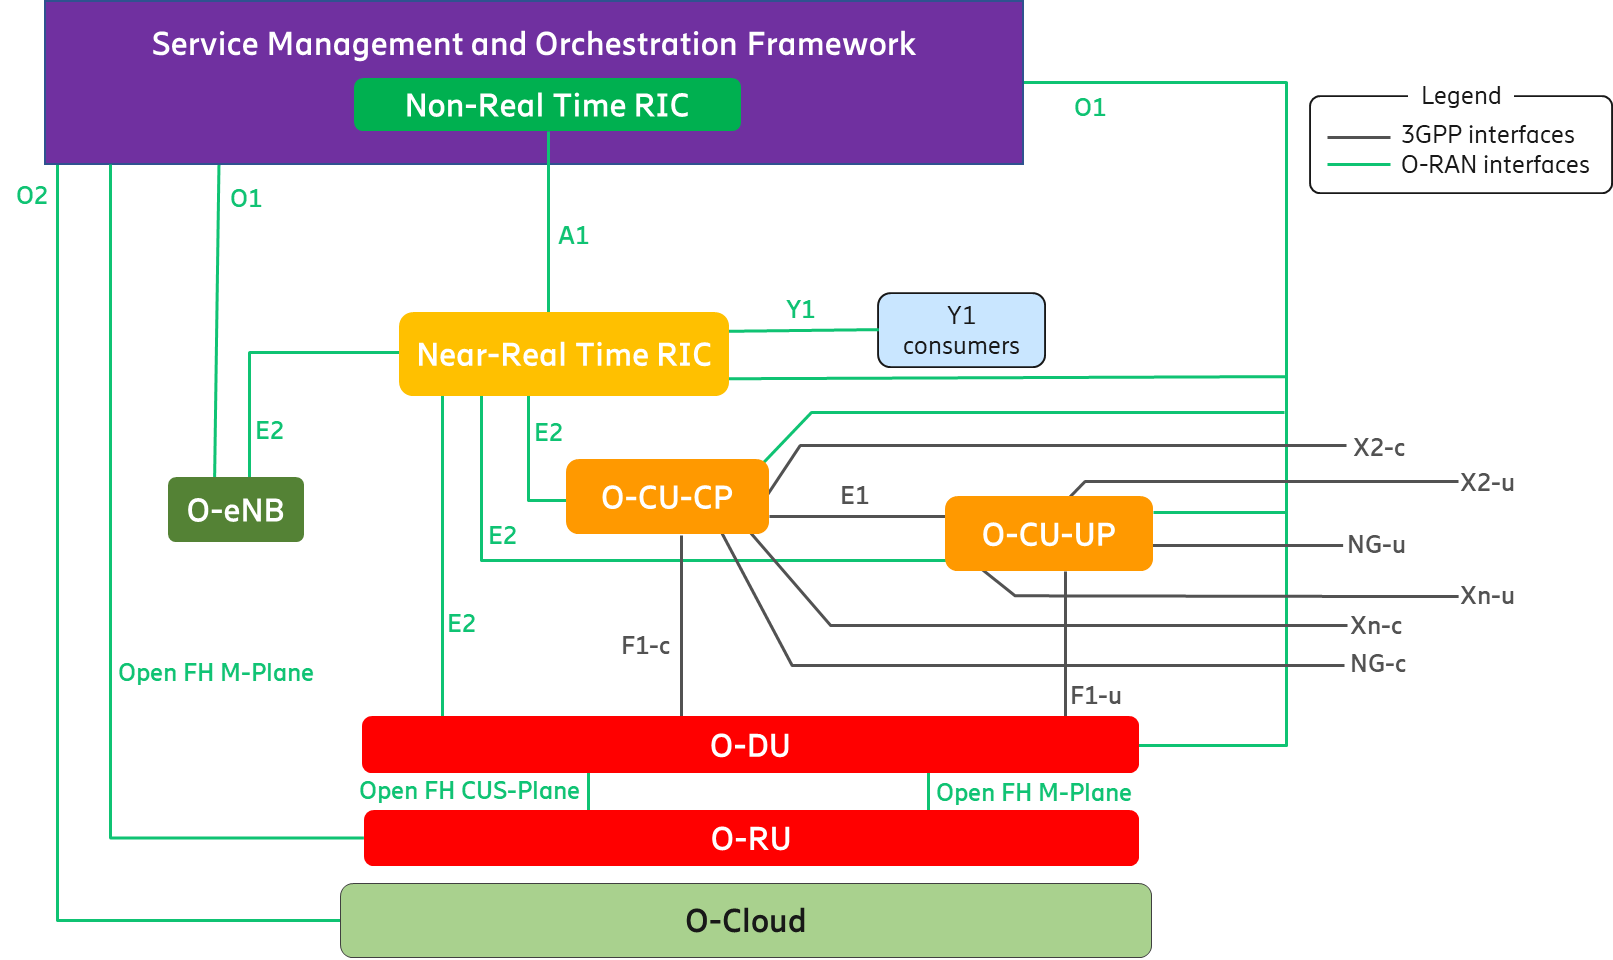
\includegraphics[width=0.8\textwidth]{oran-architecture}
    \caption{Logische Architektur von O-RAN (Quelle: \autocite{ORANAlliance})}
    \label{fig:oran-architecture}
\end{figure}

Die Architektur des O-RAN, dargestellt in Abbildung \ref{fig:oran-architecture}, wird von der \gls{wg1} verantwortet und in verschiedenen \textit{Task Groups} entwickelt. Sie basiert auf der Definition von standardisierten offenen Schnittstellen und einer logischen Trennung zwischen den Hauptfunktionen eines \glspl{ran}. Dazu gehören unter anderem der nicht-echtzeitfähige RAN-Intelligent-Controller (Non-RT-RIC) und der echtzeitfähige RIC (Near-RT-RIC), die jeweils für unterschiedliche Steuerungszyklen optimiert sind \autocite{o-ranworkgroup1usecasesandoverallarchitectureORANArchitectureDescription2024}. 

\section{Virtualisierung mit Kubernetes}
Die O-RAN \gls{sc} Referenzimplementierung basiert grundlegend auf Kubernetes, einer Plattform zur Orchestrierung von containerisierten Anwendungen \autocite{ReleaseReleasesConfluence}. Kubernetes ermöglicht es, Anwendungen in Containern auszuführen, die von ihrer Umgebung unabhängig sind und so eine hohe Flexibilität und Skalierbarkeit bieten. Container können durch Software wie Docker erstellt werden und nutzen Virtualisierung auf Betriebssystemebene, um eine isolierte Laufzeitumgebung für O-RAN Komponenten zu schaffen. Kubernetes orchestriert diese Container, indem es deren Bereitstellung, Skalierung und Verwaltung automatisiert. Das Konzept der Virtualisierung, auf dem Kubernetes aufbaut, hat zum Ziel, physische Ressourcen wie Prozessor und Arbeitsspeicher abstrahiert bereitzustellen. Dabei werden mehrere virtuelle Container auf einer physischen Maschine betrieben. Trotz der Vorteile bringt die Nutzung von Kubernetes und Virtualisierung auch Sicherheitsrisiken mit sich. Angriffsvektoren können durch falsch konfigurierte Container, ungesicherte Schnittstellen oder Schwachstellen in der Orchestrierungsplattform selbst entstehen.
Die O-RAN Spezifikation biete ein stark standardisiertes und modulares Modell, das sowohl Innovationen vorantreibt als auch Sicherheitsmaßnahmen in einem frühen Stadium der Konzeptionierung ermöglicht (\textit{security-by-design}). Die in der Literatur aufgezeigten Schwachstellen der O-RAN-\gls{sc}-Referenzimplementierung zeigen jedoch, dass erhebliche Anstrengungen nötig sind, um ein sicheres und robustes System zu gewährleisten \autocite{klementSecuringOpenRAN2024}.

\section{5G-FORAN}
\label{sec:tech-foran}
Für das Attack-Teilvorhaben wurde ein Framework implementiert, was es ermöglicht Angriffe auf die implementierte \gls{open-ran}Infrastruktur auszuführen. Dazu können verschiedene Tools genutzt werden, solange sie über eine \gls{cli} verfügen. Das Attack-Tool kann über diese Tools komplexe Angriffe simulieren und die Metadaten sowie Ergebnisse der Angriffe abspeichern. Zur Speicherung wird eine MongoDB Datenbank genutzt. MongoDB ist eine \textit{NoSQL}, dokumentenbasierte Datenbank. Ein Dokument stellt im Kontext des Attack-Tool ein Artefakt dar, welches alle relevanten Informationen über einen Angriff enthält. Diese Datenbank ist die Basis für alle Abfragen und Visualisierungen, die über das Dashboard möglich sind.
\todo{Hier noch weiterer ausführen, wenn nötig??}

\section{Dashboard}
\label{sec:tech-dashboard}
Das Dashboard ist ein Visualisierungtool, über das die Gesamtmenge aller Angriffssimulationen dargestellt werden kann. Für jeden Angriff werden die Metadaten und Ergebnisse textuell aufbereitet dargestellt und mit weiteren grafischen Visualisierungen, wie einem zeitlichen Verlauf, aufgewertet.
Das Dashboard ist über einen Webserver in der Programmiersprache \textit{Go} implementiert, der serverseitig eine Darstellung der Webseite erstellt und diese beim Aufruf der spezifischen Seiten des Dashboards an den Browser des Anwenders schickt. Neben den \gls{html} Dateien werden außerdem \gls{css} und \gls{js} Dateien ausgeliefert, die für die Weboberfläche stilisieren und Fuktionalität hinzufügen, die nicht in \gls{html} ausgedrückt werden kann. Die Architektur des Dashboard basiert auf dem Hotwire (HTML-over-the-wire) Web-Framework, welches es zum Ziel hat, möglich wenig \gls{js} einzusetzen. Stattdessen werden die \gls{html} Dateien dynamisch vom Server angepasst und in wenigen Millisekunden an den Client versandt. Dieser Ansatz ist weit verbreitet und wird auch als \textit{server-sided rendering} bezeichnet \autocite{HTMLWireHotwire}. Die einzelnen Seiten, die im Dashboard aufgerufen werden können, sind in einer Übersicht in Kapitel \ref{chap:implementierung} aufgelistet.
\todo{Hier noch weiterer ausführen, wenn nötig??}

\label{bg:mitre-frameworks}
\section{MITRE Frameworks}
Die von \gls{mitre} zur Verfügung gestellten Werkzeuge und Kategorisierungssysteme wurden entwickelt, um Sicherheitsrisiken zu analysieren, zu bewerten und zu behandeln. Die im Folgenden beschriebenen Frameworks bieten strukturierte Daten zur Analyse von Schwachstellen, Schwachstellenkategorien und Angriffsmustern. In diesem Kapitel werden die einzelnen Frameworks beschrieben und deren Anwendungsgebiete erläutert.

\subsection{MITRE ATT\&CK}
Das \gls{mitre} \gls{attack} Framework ist ein Wissensfundus, der Angreifertaktiken und -techniken dokumentiert, die auf realen Beobachtungen basieren. Es bietet eine strukturierte Möglichkeit, Angriffsmethoden zu analysieren und deren Auswirkung auf einzelne Systeme oder Infrastrukturen zu bewerten. In der aktuellen \textit{Version 16.1} enthält das Framework 14 Taktiken und 203 Techniken in der \textit{enterprise}-Matrix. Die Quelle ist aufgrund ihrer breiten Akzeptanz und der kontinuierlichen Aktualisierung durch die \gls{mitre}-Organisation als äußerst verlässlich einzustufen. \par Eine spezialisierte Erweiterung, die \gls{tm4k} von Microsoft,\todo{Hier noch auf TMK von readguard eingehen, entweder auch die abkürzung überall Ändern, auch im Dashboard.} richtet sich gezielt an Bedrohungen in containerisierten Umgebungen wie Kubernetes. Diese Matrix deckt spezifische Schwachstellen und Sicherheitsstrategien für orchestrierte Containerumgebungen ab und eignet sich deshalb auch besonders gut für Sicherheitsanalysen in \gls{open-ran}-Umgebungen \autocite{MITREATTCK,KubernetesThreatMatrix}. In der \gls{tmk} von RedGuard werden diese Techniken der Microsoft-\gls{tm4k} mit spezifischen Angriffsszenarien beschrieben.

\subsection{CAPEC}
\label{bg:capec}
Das \gls{capec} Framework zielt darauf ab, Angriffsmuster systematisch zu dokumentieren und zu klassifizieren, um Sicherheitsforscher:innen und Entwickler:innen bei der Identifikation und Vermeidung von Schwachstellen zu unterstützen. Jede \gls{capec}-Instanz beschreibt ein spezifisches Angriffsmuster, darunter die folgenden Hauptbestandteile, die für diese Arbeit besonders relevant sind:

\begin{itemize}
    \item \textbf{Angriffsmuster-ID und Name}: Eine eindeutige Kennung und Bezeichnung, die das Angriffsmuster klar identifiziert.
    \item \textbf{Beschreibung}: Eine kurze Beschreibung des Angriffs, seine Ziele und seinen Kontext.
    \item \textbf{Schwachstellenverknüpfungen}: Verweise auf relevante \glspl{cwe}, die die zugrunde liegenden Schwachstellen beschreiben, die der Angriff ausnutzt.
    \item \textbf{Taxonomie-Zuordnungen}: Verweise auf Objekte des \gls{attack} Frameworks
\end{itemize}

Die Datenbank ist umfassend und bietet eine hierarchische Klassifikation der Angriffsmuster, die es ermöglicht, zwischen allgemeinen Kategorien und spezifischen Instanzen zu navigieren. Diese Daten sind in der Sicherheitsforschung nützlich, da sie dabei helfen, typische Bedrohungen zu gruppieren und Szenarien für Sicherheitsüberprüfungen zu erstellen \autocite{CAPECCAPEC}.

\subsection{CWE}
\label{bg:cwe}
Die \gls{cwe} ist eine Aufzählung von häufigen Schwachstellenkategorien und Fehlermustern in Software und Hardware, die dazu dient, Sicherheitsprobleme systematisch zu identifizieren, zu dokumentieren und zu \autocite{CWECWE}. Jede \gls{cwe}-Instanz beschreibt eine spezifische Schwachstellenkategorie, darunter die folgenden Hauptbestandteile, die für diese Arbeit besonders relevant sind:

\begin{itemize}
    \item \textbf{Schwachstellen-ID und Name}: Eine eindeutige Kennung und Beschreibung der Schwachstellenkategorie.
    \item \textbf{Übliche Konsequenzen}: Eine Liste von typischen Auswirkungen, die durch Aunutzung einer Schwachstelle dieser Kategorie verursacht werden können.
    \item \textbf{Beobachtete Beispiele}: Verweise auf reale Anwendungsfälle, in denen ein \gls{cve} aus dieser Kategorie ausgenutzt wurde.
    \item \textbf{Demonstrative Beispiele}: Codebeispiele, die die Ausnutzung einer Schwachstelle dieser Kategorie illustrieren und deren Auswirkungen verdeutlichen.
\end{itemize}

\subsection{CVE}
\label{bg:cve}
Das \gls{cve}-System ist eine standardisierte Referenzdatenbank, die bekannte Schwachstellen und Sicherheitslücken in Software und Hardware dokumentiert. Jeder \gls{cve}-Eintrag enthält spezifische Informationen zu einer identifizierten Schwachstelle und bietet eine Grundlage für die Kommunikation und Priorisierung von Sicherheitsmaßnahmen, darunter die folgenden Hauptbestandteile, die für diese Arbeit besonders relevant sind:

\begin{itemize}
    \item \textbf{CVE-ID}: Eine weltweit eindeutige Kennung im Format \texttt{CVE-JJJJ-NNNNN}, die die Schwachstelle klar identifiziert.
    \item \textbf{Betroffene Produkte}: Angaben zu spezifischen Softwareversionen oder Hardware, die von der Schwachstelle betroffen sind.
    \item \textbf{Schweregrad und CVSS-Wertung}: Integration mit dem \gls{cvss} das, neben anderen Metriken, eine Basisbewertung von 0 bis 10 bereitstellt, um die Kritikalität der Schwachstelle zu quantifizieren.
    \item \textbf{Verknüpfungen zu CWE}: Hinweise auf zugrunde liegende Schwachstellen aus der \gls{cwe}-Taxonomie.
\end{itemize}

Das \gls{cve}-System unterscheidet sich von \gls{cwe} dadurch, dass es konkrete Sicherheitslücken in spezifischen Produkten beschreibt, während \gls{cwe} die allgemeine Kategorie oder Art der Schwachstelle adressiert. In Kombination mit \gls{capec} und \gls{cwe} ermöglicht \gls{cve} eine ganzheitliche Analyse, die sowohl Schwachstellenursachen als auch deren Ausnutzung und Abwehrmaßnahmen abdeckt. Diese Eigenschaften machen \gls{cve} zu einem unverzichtbaren Werkzeug in der Sicherheitsanalyse und ist auch sehr gut auf Open RAN-Umgebungen anwendbar, wo komplexe Architekturen eine Vielzahl potenzieller Sicherheitslücken bergen \cite{CVEWebsite}.
